\begin{figure}[htbp]
  \centering
  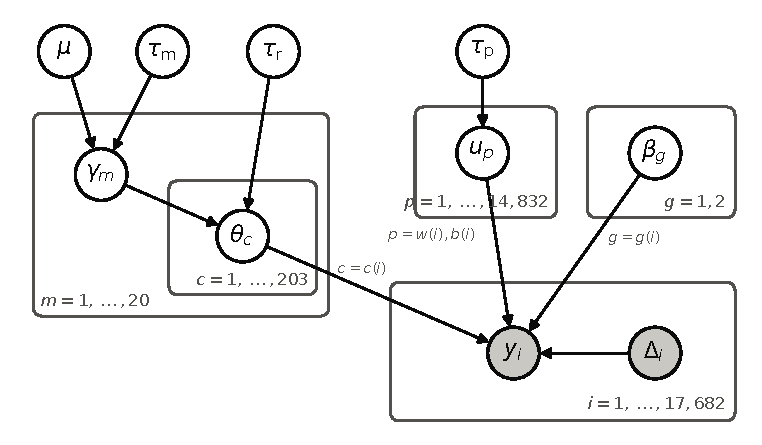
\includegraphics[width=\linewidth]{model_full.pdf}
  \caption{The final model as a Bayesian network. Shaded nodes are observed and white nodes are unknown; plates repeat their content for each of the 20 first moves $m$ of White, the 203 pairs $c$ of a first move and Black's reply (nested in their first move), the 14,832 players $p$, the two groups $g$ of rated and unrated games, and the 17,682 decisive games $i$. Game $i$ is played by White $w(i)$ against Black $b(i)$ in pair $c(i)$, in group $g(i)$; $y_i = 1$ if White wins and $0$ if Black wins, and $\Delta_i$ is the rating of White minus the rating of Black, divided by 400. $y_i \sim \text{Bernoulli}(\operatorname{logit}^{-1}(\theta_{c(i)} + \beta_{g(i)} \Delta_i + u_{w(i)} - u_{b(i)}))$, $\theta_c \sim \mathcal{N}(\gamma_{m(c)}, 1/\tau_{\mathrm{r}})$, $\gamma_m \sim \mathcal{N}(\mu, 1/\tau_{\mathrm{m}})$, $u_p \sim \mathcal{N}(0, 1/\tau_{\mathrm{p}})$, $\mu \sim \mathcal{N}(0, 0.5^2)$, $\beta_g \sim \mathcal{N}(\log 10, 1^2)$ and $\tau_{\mathrm{m}}, \tau_{\mathrm{r}}, \tau_{\mathrm{p}} \sim \text{Gamma}(1, 0.05)$ (shape and rate); we report the spreads $\sigma = 1/\sqrt{\tau}$.}
  \label{fig:model_full}
\end{figure}
